% Adjust these for the path of the theme and its graphics, relative to this file
%\usepackage{beamerthemeFalmouthGamesAcademy}
\usepackage{../../beamerthemeFalmouthGamesAcademy}
\usepackage{multimedia}
\graphicspath{ {../../} }

% Default language for code listings
\lstset{language=Python,
	morekeywords={each,in,nullptr,Bitmap,SetPixel,Color,Save,FromArgb}
}

% For strikethrough effect
\usepackage[normalem]{ulem}
\usepackage{wasysym}

\usepackage{pdfpages}

% //www.texample.net/tikz/examples/state-machine/
\usetikzlibrary{arrows,automata}

\title{\sessionnumber: Tinkering Graphics I}
\subtitle{\modulecode: \moduletitle}
\author{Michael Scott and Matt Watkins}

\setbeamertemplate{navigation symbols}{}

\newcommand{\fullbleed}[1]{
\begin{frame}[plain]
	\begin{tikzpicture}[remember picture, overlay]
		\node[at=(current page.center)] {
			\includegraphics[width=\paperwidth]{#1}
		};
	\end{tikzpicture}
\end{frame}
}

\newcommand{\picturepage}[2]{
\begin{frame}[plain]
	\begin{tikzpicture}[remember picture, overlay]
		\node[at=(current page.center)] {
			\includegraphics[width=\paperwidth]{#1}
		};
		\draw<1>[draw=none, fill=black, opacity=0.9] (-1,-5.2) rectangle (current page.south east);
		\node[draw=none,text width=0.96\paperwidth, align=right] at (5.5,-5.5) {\tiny{#2}};
	\end{tikzpicture}
\end{frame}
}

\newcommand{\notepicx}[5]{
\begin{frame}[plain]
	\begin{tikzpicture}[remember picture, overlay]
		\node[at=(current page.center)] {
			\includegraphics[width=\paperwidth]{#1}
		};
		\node[draw=none, fill=black, text width=#5\paperwidth] at ([xshift=#3, yshift=#4] current page.center) {\small{#2}};
	\end{tikzpicture}
\end{frame}
}

\newcommand{\notepic}[4]{
	\notepicx{#1}{#2}{#3}{#4}{0.4}
}

\begin{document}

\maketitle

\begin{frame}
	\frametitle{Learning Outcomes}
	By the end of this workshop, you should be able to:	
	\begin{itemize}
		\item \textbf{Apply} knowledge of colour models to \textbf{write} code that manipulates pixels in a Visual Studio Form App
		\item \textbf{Use} functions, arguments, and basic data structures such as arrays
	\end{itemize}
\end{frame}

\part{Painting with Pixels}
\frame{\partpage}

\begin{frame}
	\frametitle{Activity \#1a -- Setup}
	
	In pairs:
	
	\vspace{2em}
	
	\begin{itemize}		
		\item Open Visual Basic 
		\item Create a 'Windows Forms Application'
		\item Refer to the following documentation for details:
	\end{itemize}
\scriptsize \url{https://docs.microsoft.com/en-us/visualstudio/ide/create-csharp-winform-visual-studio}
\end{frame}

\begin{frame}[fragile]
	\frametitle{Activity \#1a -- Setup}
	
\begin{lstlisting}
int width = 640, height = 320;
Bitmap bmp = new Bitmap(width, height);

for (int y = 0; y < height; y++)
	{
	for (int x = 0; x < width; x++)
	{
		bmp.SetPixel(x, y, Color.FromArgb(255, 0, 0, 0));
	}
}
pictureBox1.Image = bmp;
bmp.Save("D:\\images\blackImage.png");
\end{lstlisting}
Note: This is an example that is contained in the 'Form' class
\end{frame}
\begin{frame}[fragile]
	\frametitle{Activity \#1a -- Setup}
	
Add a \textbf{Picturebox} from the \textbf{Toolbox} panel. Set the \textbf{Picturebox} to \textbf{Zoom}.
\center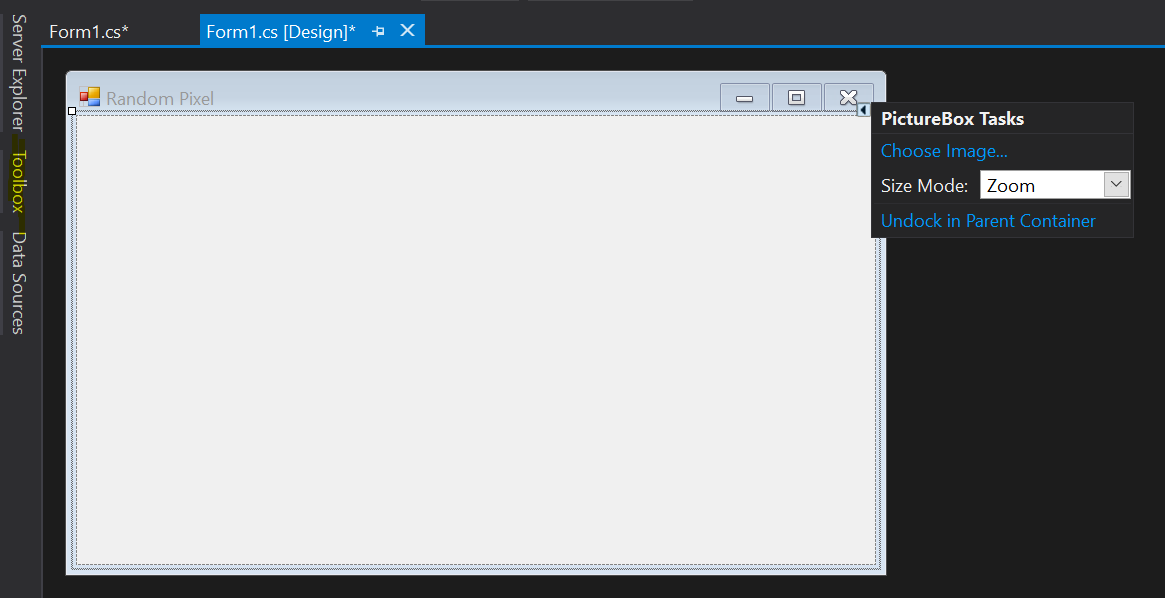
\includegraphics[scale=0.51]{initial-form-layout}
\end{frame}

\begin{frame}
		\frametitle{Key C\# Methods Used}
			\begin{itemize}		
			\item \texttt{Bitmap} - consists of the pixel data for a graphics image and its attributes.
				\begin{itemize}	
					\item \texttt{New} - Initializes a new instance of the Bitmap class with the specified size or from an existing file.
					\item \texttt{Save} - Saves the Image to the specified file or stream.
				\end{itemize}	
			\item \texttt{SetPixel} - Sets the color of the specified pixel in a Bitmap.
			\item \texttt{GetPixel} - Gets the color of the specified pixel in a Bitmap.
			\item \texttt{Color.FromArgb} - Creates a colour structure from the four 8-bit ARGB components (alpha, red, green, and blue) values.	
			\end{itemize}
\end{frame}	

\begin{frame}[fragile]
	\frametitle{Key Concepts}
	

	
	\begin{lstlisting}
for (int hours = 0; hours < 24; hours++)
{
	for (int minutes = 0; minutes < 60; minutes++)
	{
		//do something for every minute in the day
	}
}
	\end{lstlisting}
		\textbf{Nested} \texttt{for} \textbf{Loops} - to iterate through all the positions in a two dimensional array. For example: all the pixels in an image which are arranged in rows and columns.
	
\end{frame}

\fullbleed{nestedloops}
\fullbleed{nestedloops2}
\fullbleed{nestedloops3}

\begin{frame}
	\frametitle{Activity \#1b -- Setup}
	
	In pairs:
	
	\vspace{2em}
	
	\begin{itemize}		
		\item Render a green \texttt{Bitmap} image
		\item Refer to the following documentation:
		\begin{itemize}
			\item \url{https://docs.microsoft.com/en-us/dotnet/api/system.drawing.color.fromargb}
			\item \url{https://docs.microsoft.com/en-us/dotnet/api/system.drawing.bitmap.setpixel}
		\end{itemize}
	\end{itemize}
\end{frame}

\begin{frame}[fragile]
	\frametitle{Activity \#3 - Test Card}

\begin{itemize}		
	\item Create a \texttt{Bitmap} image that displays 3 equal vertical bars of red, green and blue
	\item The image must be \textbf{640 x 480} in size.
	\item Consider how you will allocate the painting of pixels to the different areas of the screen. 

\end{itemize}
	
\center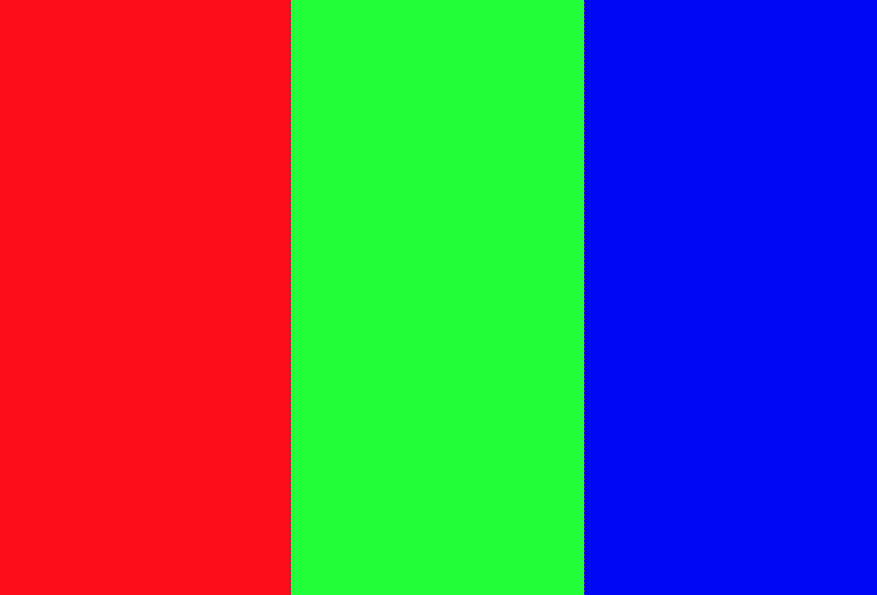
\includegraphics[scale=0.16]{testCard}

\end{frame}

\begin{frame}[fragile]
	\frametitle{Activity \#3 - Random Pixels}

\begin{itemize}		
	\item Create a \texttt{Bitmap} image that displays random pixel for every pixel in the image. Like snow on an old TV.
	\item Consider how you will generate random values for ARGB
	\item You will need to explore these methods associated with the \texttt{Random} class:
	
\end{itemize}
	
\begin{lstlisting}
 new Random();
\end{lstlisting}
Initializes a new instance of the \texttt{Random} class.
\begin{lstlisting}
Next();
\end{lstlisting}
Returns a non-negative random integer.

\end{frame}

\begin{frame}[fragile]
	\frametitle{Activity \#3 - Random Pixels}
\begin{columns}
	\column{0.48\textwidth}
	\begin{lstlisting}
Random rand = new Random();
	\end{lstlisting}
Create a variable to contain the \texttt{Random} class.
	\begin{lstlisting}
int a = rand.Next(256);
	\end{lstlisting}
Assign a variable for each colour channel and use \texttt{Next} with the new random variable to randomly choose a value.

\column{0.48\textwidth}
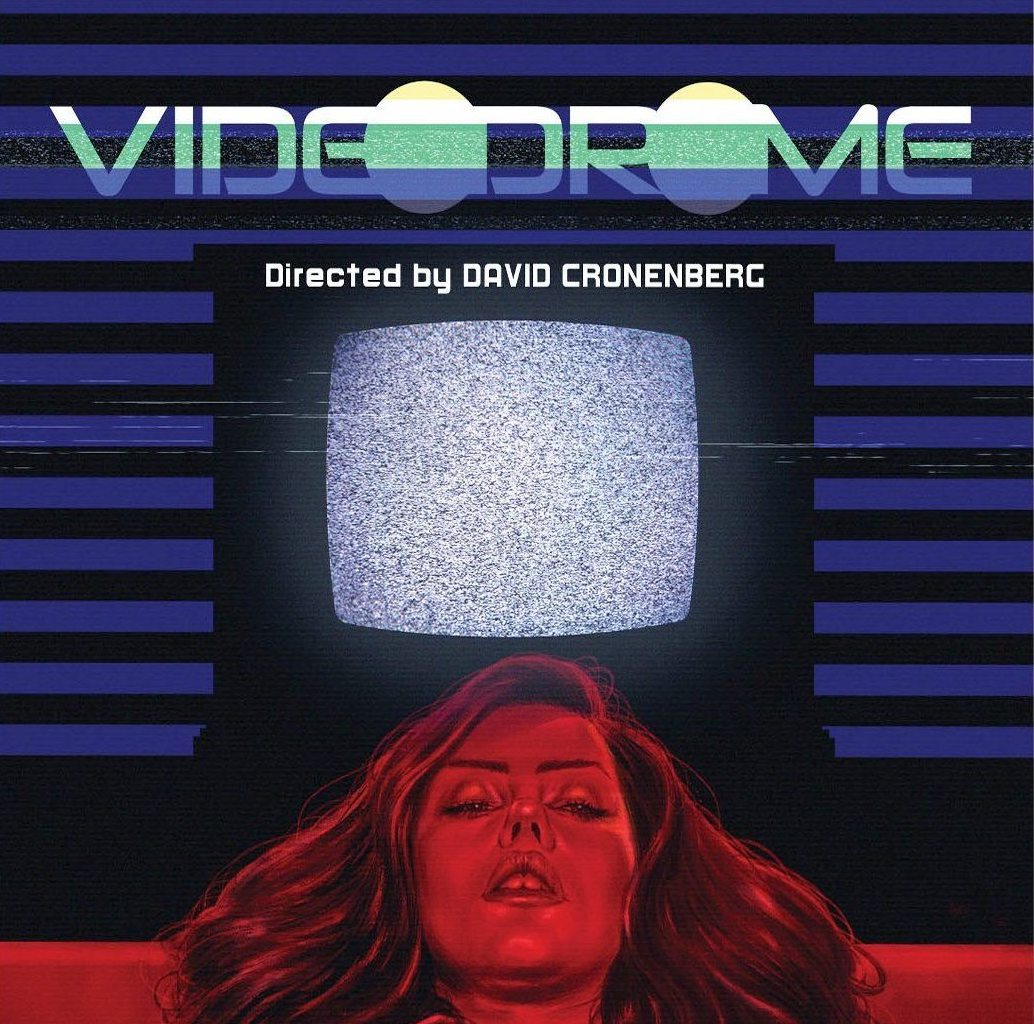
\includegraphics[scale=0.14]{videodrome}
\end{columns}
\end{frame}

\part{Manipulating Bitmaps}
\frame{\partpage}

\begin{frame}
	\frametitle{Activity \#4 -- Less Red}
	
	In pairs:
	
	\vspace{2em}
	
	\begin{itemize}		
		\item Define a function to load an image file to the Windows \texttt{Form} UI
		\item Then, define a function to reduce it's \textbf{redness}
		\item Refer to the following documentation:
		\begin{itemize}
			\item \url{https://docs.microsoft.com/en-us/dotnet/api/system.drawing.bitmap}
		\end{itemize}
	\end{itemize}
\end{frame}

\begin{frame}[fragile]
	\frametitle{Activity \#4-- Less Red}

\begin{lstlisting}
string img = "C:\\Images\\myPic.jpg";
Bitmap bmp = new Bitmap(img);
int width = bmp.Width;
int height = bmp.Height;
Bitmap rbmp = new Bitmap(bmp);

for (int y = 0; y < height; y++)
{
	for (int x = 0; x < width; x++)
	{
		Color p = bmp.GetPixel(x, y);
		int a = p.A;
		int r = p.R;
		int g = p.G;
		int b = p.B;
		int rI = Convert.ToInt32(r*.5);	
		rbmp.SetPixel(x, y, Color.FromArgb(a, rI, g, b));
	}
}
\end{lstlisting}

\end{frame}

\begin{frame}
	\frametitle{Activity \#5 -- Swap Channel}
	
	In pairs:
	
	\vspace{2em}
	
	\begin{itemize}
		\item Define a function that turns all of the red values of pixels into blue values...
		\item ...and all of the blue values into red values
	\end{itemize}
\end{frame}

\begin{frame}[fragile]
	\frametitle{Activity \#5 -- Swap Channel}
	
\begin{lstlisting}
//get pixel value
Color p = bmp.GetPixel(x, y);

//extract ARGB value from p
int a = p.A;
int r = p.R;
int g = p.G;
int b = p.B;

//swap red for blue
RtoBbmp.SetPixel(x, y, Color.FromArgb(a, r, g, r));

//swap blue for red
BtoRbmp.SetPixel(x, y, Color.FromArgb(a, b, g, b));
\end{lstlisting}

Note: This code occurs inside the nested for loop and presumes you have setup 2 bitmap variables - RtoBbmp and BtoRbmp.

\end{frame}

\begin{frame}
	\frametitle{Activity \#6 -- Greyscale}
	
	In pairs:
	
	\vspace{2em}
	
	\begin{itemize}
		\item Define a function that loads an image and turns it to greyscale
		\item Consider the following calculation:
		\begin{itemize}
			\item $New Pixel Value = \frac{\Sigma Current Channel Value}{Number Of Channels}$
		\end{itemize}
	\end{itemize}
\end{frame}

\begin{frame}[fragile]
	\frametitle{Activity \#6 -- Greyscale}
	
\begin{lstlisting}
//get pixel value
p = bmp.GetPixel(x, y);

//extract pixel component ARGB
int a = p.A;
int r = p.R;
int g = p.G;
int b = p.B;

//find average
int avg = (r + g + b) / 3;

//set new pixel value
bmp.SetPixel(x, y, Color.FromArgb(a, avg, avg, avg));
\end{lstlisting}

Note: This code occurs inside the nested for loop and presumes you have setup a bitmap variable - bmp.

\end{frame}

\begin{frame}
	\frametitle{Activity \#7 -- Negative}
	
	In pairs:
	
	\vspace{2em}
	
	\begin{itemize}
		\item Define a function that loads an image and turns it to its negative
		\item Consider the following calculation:
		\begin{itemize}
			\item $New Channel Value = 255 - Current Channel Value$
		\end{itemize}
	\end{itemize}
\end{frame}

\begin{frame}[fragile]
	\frametitle{Activity \#7 -- Negative}
	
\begin{lstlisting}
 //get pixel value
Color p = bmp.GetPixel(x, y);

//extract ARGB value from p
int a = p.A;
int r = p.R;
int g = p.G;
int b = p.B;

//find negative value
r = 255 - r;
g = 255 - g;
b = 255 - b;

//set new ARGB value in pixel
bmp.SetPixel(x, y, Color.FromArgb(a, r, g, b));
\end{lstlisting}

Note: This code occurs inside the nested for loop and presumes you have setup a bitmap variable - bmp.

\end{frame}

\begin{frame}
	\frametitle{Activity \#7 -- Top-Copy}
	
	In pairs:
	
	\vspace{2em}
	
	\begin{itemize}
		\item Define a function that copies the top half of a picture to its bottom half
		\item Refer to the following documentation:
		\begin{itemize}
			\item Consider this example of multiple conditions in a for loop as a possible solution:
			\item \url{http://www.java2s.com/Tutorial/Cpp/0060__Operators-statements/Usemultiplestatementsinforloops.htm}
		\end{itemize}
	\end{itemize}
\end{frame}

\begin{frame}[fragile]
	\frametitle{Activity \#7 -- Top-Copy}
	
	\begin{lstlisting}
int width = oldImg.Width;
int height = oldImg.Height;

Bitmap newImg = new Bitmap(width, height);

for (int y = 0, ry = height/2; y < height/2; y++, ry++)
	{
		for (int x = 0; x < width; x++ )
		{
		Color p = oldImg.GetPixel(x, y);
		newImg.SetPixel(x, y, p);
		newImg.SetPixel(x, ry, p);    
	}
}	
	\end{lstlisting}
	
	Note: You still need to consider load and saving element of this code block.
	
\end{frame}
% NEEDS REVISING FOR WEEK 3
\begin{frame}
	\frametitle{Challenge for next week -- Sunset}
	
	In pairs:
	
	\vspace{2em}
	
	\begin{itemize}
		\item Define a function that loads an image and produces several images as output, descreasing luminance
		\item You will need to think about how to reduce the luminance of the image iteratively producing a number of images and displaying them.
	\end{itemize}
\end{frame}

\begin{frame}[fragile]
	\frametitle{Challenge for next week -- Sunset}
	\begin{lstlisting}
	def decreaseRed(picture, amount):
	for p in getPixels(picture):
	value=getRed(p)
	setRed(p,value*amount)
	
	amount = 0.1 #tinker with this value
	wait_time = 50 #tinker with this value    
	
	for i in range(10):
	decreaseRed(picture, amount)
	decreaseGreen(picture, amount)
	decreaseBlue(picture, amount)
	wait(50)
	\end{lstlisting}
	Note: This is Python code can you adapt it for C\#
	
\end{frame}

\end{document}
